%%%%%%%%%%%%%%%%%%%%%%%%%%%%%% -*- Mode: Latex -*- %%%%%%%%%%%%%%%%%%%%%%%%%%%%
%% 04-15.tex -- Thesis Proposal for Ph.D
%% Author          : Hongbing Kou
%% Created On      : Mon Sep 23 11:52:28 2002
%% Last Modified By: Hongbing Kou
%% Last Modified On: Wed Nov  3 22:34:21 2004
%% RCS: $Id$
%%%%%%%%%%%%%%%%%%%%%%%%%%%%%%%%%%%%%%%%%%%%%%%%%%%%%%%%%%%%%%%%%%%%%%%%%%%%%%%
%%   Copyright (C) 2004 Hongbing Kou
%%%%%%%%%%%%%%%%%%%%%%%%%%%%%%%%%%%%%%%%%%%%%%%%%%%%%%%%%%%%%%%%%%%%%%%%%%%%%%%
%% 


\documentclass[11pt,twocolumn]{article}
\input{/export/home/csdl/tex/psfig/psfig}
\usepackage{/export/home/csdl/tex/icse2003/latex8}
\usepackage{times}
%% A verbatim-like environment which allows font changes
%%\usepackage{alltt}
%% New LaTeX2e graphics support
\usepackage[final]{graphicx}
\usepackage{url}
%% \usepackage{rotating}
% uncomment the % away on next line to produce the final camera-ready version
% and uncomment the \thispagestyle{empty} following \maketitle
\pagestyle{empty}

\begin{document}

\title{Unit Testing Development}
\author{\protect\begin{tabular}{ccc}
Hongbing Kou\\
\end{tabular}\\
\em Collaborative Software Development Laboratory\\
\em Department of Information and Computer Sciences\\
\em University of Hawai'i\\
\em Honolulu, HI, 96822\\
\em hongbing@hawaii.edu}
\maketitle
\thispagestyle{empty}

\begin{abstract}
  In software development, unit testing helps to produce working and
  reliable software. As the matter of fact unit testing can be done prior
  to, within or after code implementation. Post-coding implementation or
  execution of unit testing is well recognized because people are used to
  validation and verification mindset. Test-Driven Development (TDD)
  advocates test-first method, which means unit tests are created before
  code implementation. It is also called Test-First Design (TFD) because
  test cases are created according to requirement analyses and can
  drive code implementation as well.
  
  TDD or TFD is a highly disciplined process in that unit test is created
  according to user story iteratively and developers only write enough code
  to make tests pass in each iteration. The case studies
  \cite{George:2003}, \cite{Maximilien:2003} concluded that TDD developers
  yielded higher quality code in less time than non-TDD developers.
  However, these studies failed to address discipline issue of Test-Driven
  Development and how developers executed TDD in the experiments.
  Discipline is important because how TDD is executed can affect the
  experiment outcomes or even revert the conclusions. Another reason is
  that discipline requirements can hurdle adoption of well-defined
  processes. In my thesis I will study how developers write unit tests in
  development and TDD adoption issue.
  
  With Hackystat's assistance we can collect activities such as file
  edition, refactoring, unit test creation, test invocation so on and so
  forth. From these activities we can visualize development process
  especially unit tests creation and invocation to see how developers do
  unit test development. Once we can tell whether developers do Test-Driven
  Development or not in a period we will be able to tell whether developers
  do post-coding unit testing too. In my research I will design a
  four-iteration experiment in software engineering class to study how
  different unit testing development pattern can affect software quality
  and productivity. At first iteration students do ad-hoc unit testing
  followed by two consecutive TDD iterations. In fourth iteration students
  can choose to do TDD or not at their own wish, which helps to understand
  TDD adoption problem with the following survey.
  
  The key of this research is to figure out patterns of Test-Driven
  Development with activity data. Hackystat Eclipse sensor is already able
  to collect file editing data and refactoring activities on java objects.
  Initial activity stream and TDD viewer analyses show that we can
  visualize development process and recognize TDD stoplight pattern. Other
  TDD patterns are still yet to be categorized and quantification analysis
  on test development process is not very clear at this moment. A series of
  pilot studies on Test-Driven Development are to be conducted for pattern
  study and process quantification analysis.
  
  The milestone to accomplish this research work has three steps: I will do
  one or two pilot studies from now on to first month in spring 2005 to
  form TDD patterns and improve TDD analyses accuracy; case studies will
  span from first month of spring 2005 to the end of semester; I can
  analyze the experiment results in summer 2005 and write up thesis to
  prepare for defense in December 2005 or at an early time in 2006.

%%  Unit test plays a vital role in software development such that it's
%%  greatly emphasized not only in industry but also in software engineering
%%  education even in the introductory programming courses. It provides
%%  confidence on program for the developers and encourages changes, also can
%%  simplify system integration because of its bottom-up approach
%%  \cite{UnitTestWiki}. Usually unit tests are done by programmers in
%%  postmortem fashion to verify the correctness of programs, while
%%  Test-Driven Development proposes unit tests prior to code implementation
%%  , which changes the workflow of software development because design is
%%  postponed to and mixed with development phase. This counter-intuitive
%%  approach has been praised by many researchers and practitioners, but the
%%  lack of fine-grained process metric data makes the conclusion be
%%  questionable. One apparent question is whether the developers followed
%%  Test-Driven Development rationals or rules in the experiments.  In my
%%  thesis I will study how unit tests are written in software development
%%  and how students execute Test-Driven Development in both disciplined and
%%  freewill situations with in-process metric support from Hackystat.
\end{abstract}


\Section{Introduction}
\label{sec:intro}
  
``In computer programming, a unit test is a method of testing the
  correctness of a particular module of source code.'' \cite{UnitTestWiki}
 Unit testing is fundamental in software testing and it is at the bottom
 of software test pyramid as Figure  \ref{fig:TestLayer} shows.

  \begin{figure}[ht] 
    \centering
    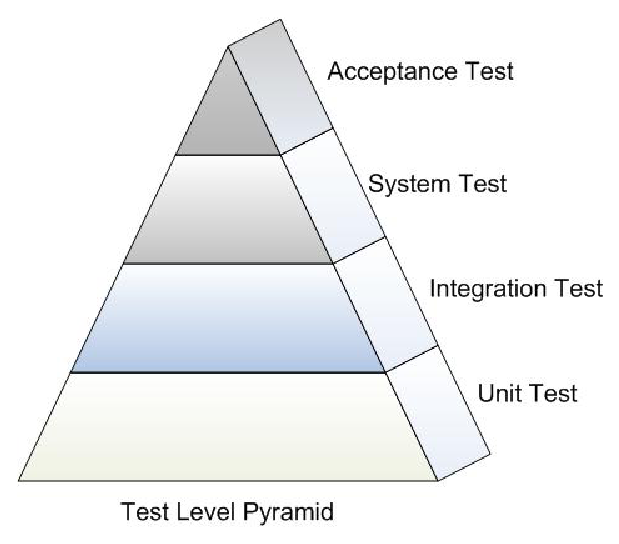
\includegraphics[width=0.5\textwidth]{TestLayerPyramid.eps}
    \caption{Software Testing Pyramid}\label{fig:TestLayer}
  \end{figure} 
 
  Usually unit testing is done by programmers themselves in postmortem
  fashion or by independant test specialists from software quality
  assurance team to find errors in the existing code. According to the cost
  model of removing bugs in different software development stages it is the
  most cost-effective way to find and remove bugs with unit tests in
  development phase. Because unit testing is good in many senses the Extreme
  Programming, one of the agile software development processes, advocates
  Test-Driven Development (TDD) as essential. In TDD unit tests are
  incrementally written prior to code implementation \cite{George:2003} and
  it drives the software design as well. If Test-Driven Development is done
  correctly you should have ideal 100\% code coverage.
  
  Some empirical case studies \cite{George:2003}, \cite{Maximilien:2003}
  reported successes on TDD practice. According to their studies TDD group
  passed more black box tests than non-TDD group and they took less time to
  finish the projects. However, there is a loophole that nobody can
  guarantee TDD developers followed TDD rationals and obeyed TDD golden
  rules strictly in the experiments. So it's unclear whether the high
  quality code is from TDD process or not. In previous cases studies there
  was no either in-process metric data or process specialists to ensure
  TDD developers obey Test-Driven Development discipline.
  
  The lack of fine-grained process data and software metrics makes it
  impossible to conclude whether developers were doing TDD, ad-hoc or test
  last in the experiments; thus, the conclusion drawn from these
  experiments become suspicious somehow. I believe addressing how unit
  testing is executed in software development can help us understand the unit
  testing effectiveness on both software quality and development
  productivity in different test paradigms, also the barrier of Test-Driven
  Development adoption.

\section{Related Work}
\label{sec:relwork}

Testing is crucial in software development because the natures of software
determine that developers can not produce perfect code that works well
every time. First of all, many software deals with large number of states
with complex algorithms. Second, system design is from customer
requirements which may have many uncertain things. And finally, the project
size may be too big such that many people are involved in the development,
which makes it more complicated \cite{Pfleeger:2001}.

Traditionally, software testing includes unit testing, system testing,
integration testing and acceptance testing \ref{fig:TestLayer}. We can see
that unit testing is at the bottom of the testing pyramid and it is
fundamental in software testing. ``The goal of unit testing is to isolate
each part of the program and show that individual parts are correct. It
provides a written contract that the piece must satisfy.''
\cite{UnitTestWiki} 

For a long run testing was thought as quality assurance specialists' job instead of
developers'. In 1996 Kent Beck, Ward Cunningham and Ron Jeffries came up
with Extreme Programming in 1996 \cite{XP96}. To support testing automation
in Extreme Programming Kent Beck proposed ``xUnit'' framework. It has the
following structure \cite{Beck:2003}:

\begin{enumerate}
\item Invoke test method
\item Invoke setUp first
\item Invoke tearDown afterward
\item Invoke tearDown even if the test method fails
\item Run multiple tests
\item Report collected results
\end{enumerate}

In recent years xUnit has already been ported to more than 30 language
supports such as JUnit for Java, PyUnit for Python, NUnit for C\#.NET,
PHPUnit for PHP, CPPUnit for C++, DUnit for Delphi etc. \cite{XPSoftware}
and it has becoming the de facto standard of unit testing in software
development. With xUnit the unit testing is shift from quality assurance
specialists to developers to improve software quality.

In extreme programming unit testing is more important than in other
software processes because all code must have unit tests and pass unit
tests before it is released \cite{XP96}. Test-Driven Development is the
extreme way to develop software in extreme programming. In TDD unit tests
are written first before implementing code. A TDD cycle is described as
following \cite{TDDWiki}:

\begin{enumerate}
\item Write the test
\item Write the code
\item Run the automated tests
\item Refactor
\item Repeat
\end{enumerate}

In TDD unit testing can not only validate the correctness of program but
also drive the design because test cases are created base on requirement
analyses. There are many researches have been done on Test-Driven
Development in both professional and educational fields. Stephen Edwards
experimented TDD in Virginia Tech in an introductory programming course in
2003 and found that TDD students did much better job than students without
TDD \cite{Edwards:04}. Boby George's study on Test-Driven Development
concluded that both students and professional TDD developers appear to have
higher code quality \cite{George:2003}. Michael Maximilien and Laurie
Williams found that defect rate of IBM Retail Core Solution project was
reduced by 50\% compared to another system built with ad-hoc unit testing
approach \cite{Maximilien:2003}, and the TDD developers passed 18\% more
functional black box tests than non-TDD developers.

Hackystat is an in-process automated metric collection system designed and
built in Collaborative Software Development Laboratory in University of
Hawaii. The attached IDE and ANT build sensors can collect the development
activities including file editing, class creation, method addition and
deletion as well as file metrics, unit test invocations, build invocations
etc. It was already used in software engineering course in University of
Hawaii and proved to be helpful in software development. The rich
in-process metrics collected by Hackystat can help us to reconstruct the
actual development process in late time without too much hassle. By
analyzing the development stream we can tell how software artifacts
are being created and the final products can be used to evaluate the
development process.

\section{Thesis Statements}
\label{sec:statement}

Developers like unit testing because it brings confidence \cite{Hunt:03} on
their code being created on a solid base and can also serve as regression
testing to check system is working or not in the new circumstance.
Everybody knows testing is important and everybody knows they don't do
enough testing \cite{Beck:00}.  In Test-Driven Development tests are
written before coding and they drive the software design as well.Initial
studies in \cite{Edwards:04}, \cite{George:2003}, \cite{Maximilien:2003}
all gave postive results on TDD; however, our experiences indicate that we
do unit testing moderately but we usually don't do TDD in Collborative
Software Development Lab and unit testing is more likely being done in
postmortem fashion. Tests are created when we don't have enough confidence
on the code being created and the continuous integration system will run
all tests automatically everyday. We believe our reluctance on TDD adoption
could be generic and with Hackystat support we will be able to find out the
reasons. Initially there are three kinds of testing styles:

\begin{enumerate}
\item Write unit tests before code, which is Test-Driven Development or
Test-First Design.
\item Write unit tests after code is written, which is used as validation. 
\item Hybrid, sometime in TDD but not exactly.
\end{enumerate}

With Hackystat in-process metric data it is feasible to categorize them and
find patterns of each. A series analyses can be created to support the
categorization and quantatively interpret the actual development process.

Previous case studies show that TDD developers yielded higher quality code
and are more productive than non-TDD developers.  An informatic survey also
found that 87.5\% of developers reported better requirement understanding
and 95.8\% of developers reported reduced debugging effort
\cite{HawleyBlog}. In my study I will revisit these claims and provide
in-process metric data to cross-validate and refine them.

\section{Methodology}
\label{sec:method}

\subsection{Graphic View of Software Process}
Software process is constructed by a series of analysis, design,
development, testing and debugging activities. It starts from requirement
analysis and ends after software products are delivered. Rational Unified
Process (RUP), Personal Software Process (PSP), Team Software Process (TSP)
and Extreme Programming (XP) are some well-defined software processes.
These processes were defined by process pioneers from their best practice
and critical thinkings on their development activities. All processes are
constructed by a set of rules and advices from requirement analyses to
testing. They exist in many kinds of software development organizations and
the rules are enforced by development team leaders or managers. Software
development process is thought as intellectual, non-repeatable and invisible.

Before delving into pattern study on test-first, test-last and hybrid unit
testing paradigms I will implement a graphic view of development process
reconstructed by development activities data collected by Hackystat
sensors. Partial functions are implemented already in TDDView to visualize
Test-Driven Development.

\subsection{Process Pattern and Quantification}
Speaking of unit testing execution in software development it could be
either test-first as specified by Test-Driven Development, test-last, or
hybid mode of test-first and test-last. In Hackystat we collect both the
development activities including implementation, compilation, unit testing
and debugging in Eclipse IDE so it is clearly feasible to study how unit
tests are implemented in the development process. Software process rules
can be used to generate development patterns to categorize how developers
do unit testing in the real implementation. One thought here is to design a
rule-based agent to study the development pattern [further research to be
conducted] to do the categorization.

\subsection{Experiments Design}
To study thesis claims we propose an iterative experiment in software
engineering class in spring 2005.

\begin{enumerate}
\item At beginning of class students will learn advanced java development
  skills for class projects including Eclipse IDE, JUnit, ANT, Hackystat
  and so forth. Some assignments will be given to students to practice new
  skills, configure development environment setting and utilize their
  Hackystat data.
\item Students start working on their own projects individually in this
  round. Unit testing is encouraged but not demanded.
\item We introduce Test-Driven Development to students and ask them to try
  to do Test-Driven Development. To enourage TDD adoption we will use the
  process graphic viewer and quantification anlaysis to give extra
  credit. 
\item Based on feedback and problem analysis in TDD development in the last
  iteration students will gain better understanding to TDD development. We
  still encourage them to use TDD at this step.
\item In the last round students have the choice to do TDD, test last or
  hybrid.
\end{enumerate}

Apparently we need to have students' Hackystat data to study how unit
testing is executed is executed in the development to prove or disprove our
claims on Test-Driven Development.

\section{Conclusion and Discussion}
\label{sec:discuss}

To Be Done.
\bibliography{/export/home/csdl/bib/tdd,/export/home/csdl/bib/csdl-trs}
\bibliographystyle{plain}

\end{document}









































































